\documentclass[10pt]{article}

% Manage page layout
\usepackage[margin=2.5cm, includefoot, footskip=30pt]{geometry}
\pagestyle{plain}
\setlength{\parindent}{0em}
\setlength{\parskip}{1em}
\renewcommand{\baselinestretch}{1}

%%%%%%%PACKAGES HERE%%%%%%%
\usepackage{tikz}
\usepackage{amsmath}
\usepackage{amssymb}
\usepackage{graphicx}
\usepackage{subcaption}
\usepackage{standalone}
\usepackage{algorithm, setspace}
\usepackage[noend]{algpseudocode}

\makeatletter
\def\BState{\State\hskip-\ALG@thistlm}
\makeatother

\newcommand{\R}{\mathbb{R}}
\newtheorem{theorem}{Theorem}
\usetikzlibrary{decorations.pathmorphing, decorations.pathreplacing, angles,
                quotes, calc, er, positioning}

\newtheorem{lemma}[theorem]{Lemma}
%%%%%%%%%%%%%%%%%%%%%%%%%%%
\title{Memory size in the Prisoner's Dilemma}
\author{Nikoleta E. Glynatsi \and Vincent Knight}
\date{}

\begin{document}

\maketitle

\begin{abstract}

In this manuscript we build upon a framework provided in 1989 for the study of
these strategies and identify the best responses of memory one players. The aim
of this work is to show the limitations of memory one strategies in multi-opponent
interactions. A number of theoretic results are presented.
%TODO: Expand when we get results
\end{abstract}

\section{Introduction}\label{section:introduction}

The Prisoner's Dilemma (PD) is a two player person game used in understanding the
evolution of co-operative behaviour. Each player can choose between cooperation
(C) and defection (D). The decisions are made simultaneously and independently.
The normal form representation of the game is given by:

\begin{equation}\label{equ:pd_definition}
    S_p = \begin{pmatrix}
    R & S  \\
    T & P
    \end{pmatrix} \quad
    S_q = \begin{pmatrix}
        R & T  \\
        S & P
        \end{pmatrix}
\end{equation}

where \(S_p\) represents the utilities of the first player and \(S_q\) the utilities
of the second player. The payoffs, \((R, P, S, T)\), are constrained by equations
(\ref{eq:pd_constrain_one}) and~(\ref{eq:pd_constrain_two}). Constrain
(\ref{eq:pd_constrain_one}) ensures that defection dominates cooperation and
constrain (\ref{eq:pd_constrain_two}) ensures that there is a dilemma. Because
the sum of the utilities for both players is better when both choose cooperation.
The most common values used in the literature are \((3, 1, 0, 5)\)~\cite{Axelrod1981}.

\begin{equation}\label{eq:pd_constrain_one}
    T > R > P > S 
\end{equation}

\begin{equation}\label{eq:pd_constrain_two}
    2R > T + S
\end{equation}

The PD is a one shot game, however it is commonly studied in a manner where the
history of the interactions matters. The repeated form of the game is called the
Iterated Prisoner's Dilemma (IPD) and in the 1980s following the work of
\cite{Axelrod1980a, Axelrod1980b} it attracted the attention of the scientific
community.

In~\cite{Axelrod1980a} a computer tournament of the IPD was performed. A
tournament is a series of rounds of the PD between pairs of strategies. The
topology commonly used, \cite{Axelrod1980a, Axelrod1980b}, is that of a round
robin where all contestants compete against each other. The winner of these
tournaments was decided on the average score and not in the number of wins.

These tournaments were the milestones of an era which to today is using
computer tournaments to explore the robustness of strategies of IPD.
The robustness can also be checked through evolutionary process~\cite{Nowak}.
However, this aspect will not be considered here, instead the focus is on
performance in tournaments.

In Axelrod's original tournaments \cite{Axelrod1980a, Axelrod1980b}, strategies
were allowed access to the history and in the first tournament they also knew
the number of total turns in each interaction. The history included the
previous moves of both the player and the opponent. How many turns of history
that a strategy would use, the memory size, was left to the creator of the
strategy to decide. For example the winning strategy of the first tournaments,
Tit for Tat was a strategy that made use of the previous move of the opponent
only. Tit for Tat is a strategy that starts by cooperating and then mimics the
previous action of it's opponent. Strategies like Tit for Tat are called memory
one strategies. A framework for studying memory one strategies was introduced
in~\cite{Nowak1989} and further used in~\cite{Nowak1993, Nowak1990}.

In~\cite{Press2012} Press and Dyson, introduced a new set of memory one
strategies called zero determinant (ZD) strategies. The ZD strategies,
manage to force a linear relationship between the score of the strategy
and the opponent. Press and Dyson, prove their concept of the ZD strategies
and claim that a ZD strategy can outperform any given opponent.

The ZD strategies have tracked a lot of attention. It was stated that
``Press and Dyson have fundamentally changed the viewpoint on the Prisoner's
Dilemma''~\cite{Stewart2012}. In~\cite{Stewart2012}, the Axelrod's
tournament have been re-run including ZD strategies and a new set of ZD
strategies the Generous ZD. Even so, ZD and memory one strategies have
also received criticism. In~\cite{Harper2015}, the `memory of a strategy does
not matter' statement was questioned. A set of more complex strategies,
strategies that take in account the entire history set of the game, were
trained and proven to be more robust than ZD strategies.

\section{Problem}

The purpose of this work is to consider a given memory one strategy 
in a similar fashion to~\cite{Press2012}. However whilst~\cite{Press2012} found
a way for a player to manipulate an opponent, this work will consider an
optimisation approach to identify the best response to that opponent.
In essence the aim is to produce a compact method of identifying the best memory
one strategy against a given opponent.

The second part of this manuscript we explore the limitation of the best response
memory one strategies by comparing them to more complex strategies with a larger
memory.

\subsection{Background}

In this manuscript we explore the robustness of memory one strategies.
A memory one strategy is defined as a strategy that decides it's action in turn
\(m\) based on what occurred in turn \(m - 1\). If a strategy is concerned with
only the outcome of a single turn then there are four possible `states' the
strategy could be in. These are \(CC, CD, DC,CC\). A memory one strategy is denoted
by the probabilities of cooperating after each of these states,
\(p=p_1, p_2, p_3, p_4 \in \R_{[0,1]} ^ 4\). A diagrammatic representation of
such as strategy is given in Figure~\ref{fig:diagram_mem_one}.

\begin{figure}
    \centering
    \begin{subfigure}{0.45\textwidth}
        \centering
        \includestandalone[width=.65\textwidth]{tex/states}
        \subcaption{Diagrammatic representation of a memory one strategy.}
        \label{fig:diagram_mem_one}
    \end{subfigure}
    \begin{subfigure}{0.45\textwidth}
        \centering
        \includestandalone[width=.88\textwidth]{tex/markov_chain}
        \subcaption{Markov chain on a PD game.}
        \label{fig:markov_chain}
    \end{subfigure}
\end{figure}

In~\cite{Nowak1990} a framework was introduced to study the interactions of memory
one strategies modelled as a stochastic process, where the players move from one
of the states \(CC, CD, DC,CC\) to another. More specifically, it can be modelled
by the use of a Markov process of four states, shown by Figure~\ref{fig:markov_chain}.

The transition matrix of the markov chain in Figure~\ref{fig:markov_chain}
is defined as \(M\) and is given by,

\begin{equation}\label{eq:m_matrix}
    M = \left[\begin{matrix}p_{1} q_{1} & p_{1} \left(- q_{1} + 1\right) & q_{1} \left(- p_{1} + 1\right) & \left(- p_{1} + 1\right) \left(- q_{1} + 1\right)\\p_{2} q_{3} & p_{2} \left(- q_{3} + 1\right) & q_{3} \left(- p_{2} + 1\right) & \left(- p_{2} + 1\right) \left(- q_{3} + 1\right)\\p_{3} q_{2} & p_{3} \left(- q_{2} + 1\right) & q_{2} \left(- p_{3} + 1\right) & \left(- p_{3} + 1\right) \left(- q_{2} + 1\right)\\p_{4} q_{4} & p_{4} \left(- q_{4} + 1\right) & q_{4} \left(- p_{4} + 1\right) & \left(- p_{4} + 1\right) \left(- q_{4} + 1\right)\end{matrix}\right].
\end{equation}

Let the vector of the stationary probabilities of \(M\) be defined as \(v\).
Vector \(v\) are given in the Appendix. %TODO include Appendix
The scores of each player can be retrieved by multiplying the probabilities of each
state, at the stationary state, with the equivalent payoff. Thus, the  utility for
player \(p\) against \(q\), denoted as \(u_q(p)\), is defined by,

\begin{equation}\label{eq:press_dyson_utility}
    u_q(p) = v \times S_p.
\end{equation}

\subsection{Utility}

The analytical formulation gives the advantage of time. That is because the 
payoffs of a match between two opponents are now retrievable without 
simulating the actual match itself.

Note though that \(u_q(p)\) is a function of 4 variables which is also affected
by the transition probabilities of the opponent \(q\). The first theoretical
result that we introduce in this work is a compact way of writing \(u_q(p)\).
This is given by the Theorem~\ref{theorem:quadratic_form_u}.

\begin{theorem}\label{theorem:quadratic_form_u}
    For a given memory one strategy \(p\in\mathbb{R}_{[0,1]}^4\) playing another 
    memory one strategy \(q\in\mathbb{R}_{[0,1]}^4\), the 
    utility of the player \(u_q(p)\) can be re written as a ratio of two quadratic
    forms:
    
    \begin{equation}\label{eq:optimisation_quadratic}
    u_q(p) = \frac{\frac{1}{2}p^TQp + c^Tp + a}
                {\frac{1}{2}p^T\bar{Q}p + \bar{c}^Tp + \bar{a}}, 
    \end{equation}
    where \(Q, \bar{Q}\) are matrices of \(4 \times 4\) defined with the transition
    probabilities of the opponent's transition probabilities \(q_1, q_2, q_3, q_4\).
    
    \begin{center}
    \begin{equation}
    \resizebox{0.9\linewidth}{!}{\arraycolsep=2.5pt%
    \boldmath\(
    Q = \left[\begin{matrix}0 & 5 q_{4} \left(q_{1} - q_{3}\right) & - q_{4} \left(q_{1} - q_{2}\right) & \left(q_{1} - q_{4}\right) \left(q_{2} - 5 q_{3} - 1\right)\\5 q_{4} \left(q_{1} - q_{3}\right) & 0 & - 3 q_{4} \left(q_{2} - q_{3}\right) & \left(q_{3} - q_{4}\right) \left(5 q_{1} - 3 q_{2} - 2\right)\\- q_{4} \left(q_{1} - q_{2}\right) & - 3 q_{4} \left(q_{2} - q_{3}\right) & 0 & - \left(q_{2} - q_{4}\right) \left(q_{1} - 3 q_{3} - 1\right)\\\left(q_{1} - q_{4}\right) \left(q_{2} - 5 q_{3} - 1\right) & \left(q_{3} - q_{4}\right) \left(5 q_{1} - 3 q_{2} - 2\right) & - \left(q_{2} - q_{4}\right) \left(q_{1} - 3 q_{3} - 1\right) & 0\end{matrix}\right]\)},
    \end{equation}
    \begin{equation}\label{eq:q_bar_matrix}
    \resizebox{0.8\linewidth}{!}{\arraycolsep=2.5pt%
    \boldmath\(
    \bar{Q} =  \left[\begin{matrix}0 & - \left(q_{1} - q_{3}\right) \left(q_{2} - q_{4} - 1\right) & \left(q_{1} - q_{2}\right) \left(q_{3} - q_{4}\right) & \left(q_{1} - q_{4}\right) \left(q_{2} - q_{3} - 1\right)\\- \left(q_{1} - q_{3}\right) \left(q_{2} - q_{4} - 1\right) & 0 & \left(q_{2} - q_{3}\right) \left(q_{1} - q_{4} - 1\right) & \left(q_{1} - q_{2}\right) \left(q_{3} - q_{4}\right)\\\left(q_{1} - q_{2}\right) \left(q_{3} - q_{4}\right) & \left(q_{2} - q_{3}\right) \left(q_{1} - q_{4} - 1\right) & 0 & - \left(q_{2} - q_{4}\right) \left(q_{1} - q_{3} - 1\right)\\\left(q_{1} - q_{4}\right) \left(q_{2} - q_{3} - 1\right) & \left(q_{1} - q_{2}\right) \left(q_{3} - q_{4}\right) & - \left(q_{2} - q_{4}\right) \left(q_{1} - q_{3} - 1\right) & 0\end{matrix}\right]\)}.
    \end{equation}
    \end{center}
    
    \(c \text{ and } \bar{c}\), are \(4 \times 1\) vectors defined by the transition rates 
    \(q_1, q_2, q_3, q_4\).
    
    \begin{equation}\label{eq:q_matrix_numerator}
    \resizebox{0.3\linewidth}{!}{\arraycolsep=2.5pt%
    \(c = \left[\begin{matrix}- 5 q_{1} q_{4}\\5 q_{4} \left(q_{3} - 1\right)\\q_{4} \left(2 q_{2} + 1\right)\\5 q_{1} q_{4} - 2 q_{2} q_{4} - q_{2} - 5 q_{3} q_{4} + 5 q_{3} - 3 q_{4} + 1\end{matrix}\right]\),}
    \end{equation}
    \begin{equation}\label{eq:q_matrix_denominator}
    \resizebox{0.3\linewidth}{!}{\arraycolsep=2.5pt%
    \(\bar{c} = \left[\begin{matrix}q_{1} \left(q_{2} - q_{4} - 1\right)\\- \left(q_{3} - 1\right) \left(q_{2} - q_{4} - 1\right)\\- q_{1} q_{2} + q_{2} q_{3} + q_{2} - q_{3} + q_{4}\\q_{1} q_{4} - q_{2} - q_{3} q_{4} + q_{3} - q_{4} + 1\end{matrix}\right]\).
    }
    \end{equation}
    
    Lastly, \(a = 5 q_{4}\) and 
    \(\bar{a} = - q_{2} + q_{4} + 1\).
    \end{theorem}

\subsection{Validation}

In this section we validate the formulation of Theorem~\ref{theorem:quadratic_form_u}
using numerical experiments. All the simulated results of this work are done
using~\cite{axelrodproject} which is an open research framework for the study of
the IPD. This package is described in~\cite{Knight2016}.

To validate the formulation of \(u_q(p)\) several memory one players were 
matched against 20 opponents.The simulated value of \(u_q(p)\) has been calculated
using \cite{axelrodproject} and the theoretical by  substituting in equation~(\ref{eq:optimisation_quadratic}).

In Figure~\ref{fig:analytical_simulated}, both the simulated and the theoretical
value of \(u_q(p)\), against each opponent, are plotted for three different memory
one strategies. Figure \ref{fig:analytical_simulated} indicates that the 
formulation of \(u_q(p)\) as a quadratic ratio successfully captures the 
simulated behaviour.

\begin{figure}[!htbp]
\begin{center}
    \begin{subfigure}{0.45\textwidth}
        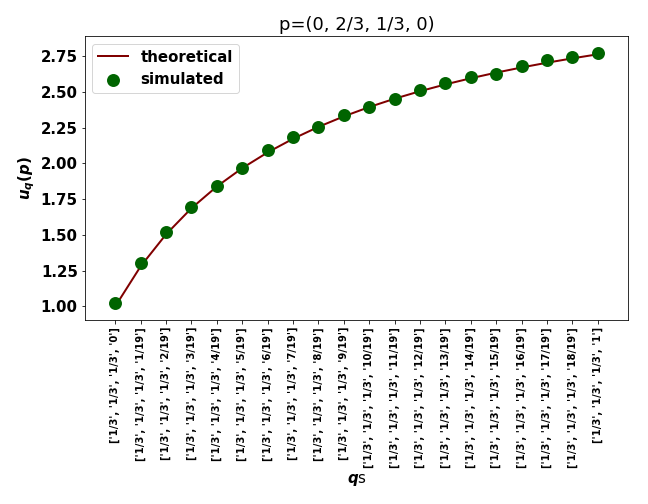
\includegraphics[width=\linewidth]{img/validation_img_two.png}
    \end{subfigure}
    \begin{subfigure}{0.45\textwidth}
        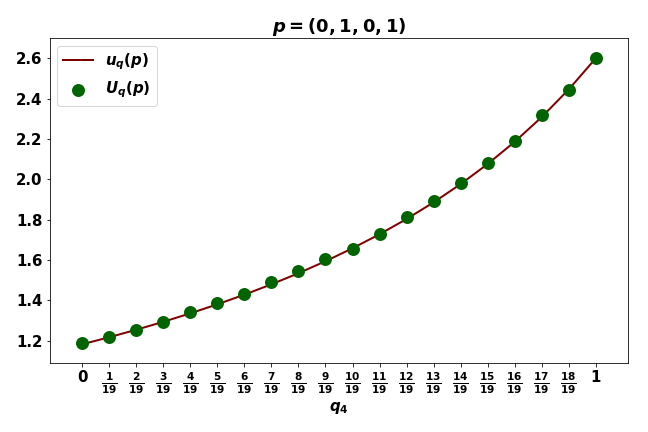
\includegraphics[width=\linewidth]{img/validation_img_three.png}
    \end{subfigure}
\end{center}
\caption{Differences between simulated and analytical results.}
\label{fig:analytical_simulated}
\end{figure}

\section{Best responses Analytically}

In the introduction a question was raised: which memory one strategy is the \textbf{best response}
against another memory one? This will be considered as an optimisation problem,
where a memory one strategy \(p\) wants to optimise it's utility \(u_q(p)\)
against an opponent \(q\). The decision variable is the vector \(p\) and the
solitary constrains \(p \in \R^4_{[0, 1]} \). The optimisation problem is
given by~(\ref{eq:mo_optimisation}).

\begin{equation}\label{eq:mo_optimisation}
\begin{aligned}
& \max_p: && \frac{\frac{1}{2}  p  Q  p^T + c^T p + a} 
                  {\frac{1}{2}  p  \bar{Q}  p^T + \bar{c}^T  p + \bar{a}}
\\
& \text{such that}: && \ p \in \R^4_{[0, 1]}.
\end{aligned}
\end{equation}

\subsection{Convexity}

This work is concerned with a fractional optimisation problem of quadratic forms.
Initially, the convexity, whether or not \(u_{q}(p)\) is concave~\cite{Gradshteyn2007},
will be checked (concave because is a maximisation  problem).

To test the hypothesis that \(u_q(p)\) is concave an empirical analysis
was performed using computer code. %TODO add the data generated
It was shown that there exists at least one point for which the definition of
concavity does not hold. Optimising a non concave function is rather tricky.

Several articles in fractional optimisation of quadratic forms that was non concave
can be found~\cite{Beck2009, Hongyan2014}. Though in these works both the numerator
and denominator of the fractional problem were concave. In~\cite{Anton2014} it is
stated that a quadratic form will be concave if and only if it's symmetric matrix is
negative semi definite.

In Appendix, it is proved that neither the numerator or the denominator of
equation~(\ref{eq:optimisation_quadratic}) are concave.

\subsection{Proof}

The non concavity of \(u(p)\) indicates multiple local optimal points. Thus a
compact way of searching the candidate optimal points needs to be introduced.
Once the method is defined then the utility of each point is compared to the
rest. The optimal point is the point that has the highest value of \(u(p)\).

The problem considered is a bounded, this mean that the we know that the candinate solutions
will be either on the bounds of our feasable solution in a point in the center.
Note that the points are the roots of the derivate \(\frac{du}{dp}\). Bound case are all
the possible combinations of \(p_1, p_2, p_3, p_4 \in \{0, 1\}\). Figure~\ref{fig:cube}
illustrates an example of possible locations of candidate solutions for a 3 dimensional
problem.

\begin{figure}
\begin{center}
    \includestandalone[width=\textwidth]{tex/cube}
    \caption{Candidate solution of a 3 dimensional problem.}\label{fig:cube}
\end{center}
\end{figure}

The derivate \(\frac{du}{dp}\) is given by,

\begin{equation}\label{eq:derivative_of_quadratic}
    \begin{aligned}
     \frac{du}{dp} & = && \frac{(  \frac{1}{2}p  Q  p^T + c^T p + a)'
      (  \frac{1}{2} p  \bar{Q}  p^T + \bar{c}^T  p + \bar{a}) - 
      (  \frac{1}{2} p  \bar{Q}  p^T + \bar{c}^T  p + \bar{a})'
      (  \frac{1}{2} p  Q  p^T + c^T p + a)}
      {(  \frac{1}{2} p  \bar{Q}  p^T + \bar{c}^T  p + \bar{a})^2} \\
      \\
    & = && \frac{(pQ + c^T) ( \frac{1}{2} p  \bar{Q}  p^T + \bar{c}^T  p + \bar{a}) 
    - (p\bar{Q} + \bar{c}^T)( \frac{1}{2} p  Q  p^T + c^T p + a)}
      {( \frac{1}{2} p  \bar{Q}  p^T + \bar{c}^T  p + \bar{a})^2} \\
    \end{aligned}
\end{equation}

Thus we conclude that the best response of a memory one strategy in matchs is
given by Lemma~\ref{lemma:memone_best_response}.

\begin{lemma}\label{lemma:memone_best_response}
    The optimal behaviour of a memory one strategy player \((p^*)\) against a
    given opponent \(q\) is given by:
    
    \[p^* = \textnormal{argmax}(u_q(p)), \ p \in S_q,\]
    
    where the set \(S_q\) is defined as 
    
    \[S_q = \{0, \bar{p}, 1 \}^4 \]
    
    where the vector \(\bar{p}\) is the vector for which the following condition is true:
    
    {\small
    \begin{equation*}
        (pQ + c^T) ( \frac{1}{2} p  \bar{Q}  p^T + \bar{c}^T  p + \bar{a}) 
        - (p\bar{Q} + \bar{c}^T)( \frac{1}{2} p  Q  p^T + c^T p + a) = 0
    \end{equation*}}

    Note that this is a \(4-\) polynomial system of \(4\) variables. Each polynomial
    corresponds to a partial derivative of \(u_q(p)\).
\end{lemma}

The method of Lagrange Multipliers and Karush-Kuhn-Tucker conditions has also been
applied and reached the same conclusion. %TODO add reference.
The Karush-Kuhn-Tucker conditions are used becase ourconstrains are inequalities.

A question that arises immediately after the work that has been carried out to
this point is the following: What is the optimal memory player against multiple
opponents, in a tournament environment.

Let us consider a collection of opponents: \(\{q^{(1)}, q^{(2)}, \dots, q^{(N)}\}\), 
finding the optimal behaviour of a strategy can now be written as:

\begin{equation}\label{eq:random_tournament_optimisation}
\begin{aligned}
\max_p: & \ \frac{1}{N} \sum_{i=1} ^ {N} {u_q}^{(i)} (p) 
\\
st: & \ p_1 = p_2 = p_3 = p_4 = p\\
    & \ p \in \R_{[0, 1]} 
\end{aligned}
\end{equation}

Thus, the average utility against a set of opponents is maximised and the average 
utility is given by,

\begin{equation}\label{eq:tournament_utility}
    \frac{1}{N} \sum\limits_{i=1} ^ {N} {u_q}^{(i)} (p) = \frac{1}{N}
    \frac{\sum\limits_{i=1} ^ {N} (\frac{1}{2} pQ^{(i)} p^T + c^{(i)T} p + a^ {(i)})
    \prod\limits_{\tiny\begin{array}{l} j=1 \\ j \neq i \end{array}} ^ 
    N (\frac{1}{2} p\bar{Q}^{(i)} p^T + \bar{c}^{(i)T} p + \bar{a}^ {(i)})}
    {\prod\limits_{i=1} ^ N (\frac{1}{2} p\bar{Q}^{(i)} p^T + \bar{c}^{(i)T} p + \bar{a}^ {(i)})}.
\end{equation}

If we were to follow a similar approach to that of pairwise interactions the derivative
of the utility would be calculated and set to zero. Furthemore, the bound cases would
we explored. The derivate of the average utility is given by,

{\scriptsize
\begin{align*}
    \frac{d}{dp} \frac{1}{N} \sum\limits_{i=1} ^ {N} {u_q}^{(i)} (p) & = \\
    & =\frac{
    (\sum\limits_{i=1} ^ {N} Q_{N}^{(i)'} \prod\limits_{\tiny\begin{array}{l} j=1 \\ j \neq i \end{array}} ^ N Q_{D}^{(i)}
    + \sum\limits_{i=1} ^ {N} Q_{D}^{(i)'} \sum\limits_{\tiny\begin{array}{l} j=1 \\ j \neq i \end{array}} ^ {N} Q_{N}^{(i)}
    \prod\limits_{\tiny\begin{array}{l} l=1 \\ l \neq i \ \\ l \neq j \end{array}} ^ N Q_{D}^{(i)}) \times
    \prod\limits_{i=1} ^ N Q_{D}^{(i)} - (\sum\limits_{i=1} ^ {N} Q_{D}^{(i)'}
    \prod\limits_{\tiny\begin{array}{l} j=1 \\ j \neq i \end{array}} ^ N Q_{D}^{(i)}) \times 
    (\sum\limits_{i=1} ^ {N} Q_{N}^{(i)} \prod\limits_{\tiny\begin{array}{l} j=1 \\ j \neq i \end{array}} ^ N Q_{D}^{(i)})}
    {(\prod\limits_{i=1} ^ N Q_{D}^{(i)})^{2}}
\end{align*}
}
where,

\begin{align*}
    Q_{N}^{(i) } & = \frac{1}{2} pQ^{(i)} p^T + c^{(i)T} p + a^ {(i)}, \\
    Q_{N}^{(i)'} & =  pQ^{(i)} + c^{(i)T}, \\
    Q_{D}^{(i) } & = \frac{1}{2} p\bar{Q}^{(i)} p^T + \bar{c}^{(i)T} p + \bar{a}^ {(i)}, \\
    Q_{D}^{(i)'} & =  p\bar{Q}^{(i)} + \bar{c}^{(i)T}. \\
\end{align*}

Note that neither problems can be further handled analytically. For pairwise
interactions, the roots of the derivate are given by solving a multivariare \(4-\)
system of \(4-\) variables. The problem's size is gradually increasing every time
an extra opponent is taken into account.

Thus no further analytical consideration is given to these problem in this work.
In the following sections numerical methods are introduced which will be used to
discover best responses. Moreover, several constrain versions of our problem
and their exact solutions are discussed.

\section{Numerical Experiments}

In this section we introcude several numerical methods to supplement our analytical
approach.

Initally, several insights and exact methods considered in this work to identify
best responses in further constained problems are discussed. These further
constrained problems taken into account subsets of memeory one strategies, which
are

\begin{itemize}
    \item purely random strategies
    \item reactive strategies.
\end{itemize}

Purely random strategies are a set of memory one strategies where the transition
probabilities of each state are the same. The optimisation problem of (\ref{eq:mo_optimisation})
now has an extra constraint and is re written as,

\begin{equation}\label{eq:random_optimisation}
\begin{aligned}
\max_p: & \ u_q(p)
\\
\text{such that}: & \ p_1 = p_2 = p_3 = p_4 = p\\
    & \ 0 \leq p \leq 1. 
\end{aligned}
\end{equation}

The utility for a random player is now a function of a signle unknown. For the
random player in an \(N\) interactions enviroment the folliwing algorithm allow us to
retrieve the exact best responose.

\begin{algorithm}
    \setstretch{1.35}
    \caption{Best response algorithm for purely random strategies}\label{algo:purely}
    \begin{algorithmic}[1]
    \Procedure{Purely random search}{}
    \State $N \gets \text{number of opponets}$ 
    \State $S_q \gets \{0, 1\}$ 
    \BState \emph{loop} $i=1 \text{ to } 2N$:
    \State $S_q \cup \bar{p}_{i} \text{ for } \frac{du}{d\bar{p}_{i}} = 0$.
    \State $i \gets i + 1$.
    \State \textbf{goto} \emph{loop}.
    \State \textbf{close};
    \State $p^* \gets \text{argmax}(u_q (p)), p \in S_q $.
    \EndProcedure
    \end{algorithmic}
    \end{algorithm}

Numerical experiments are perform and they suggest that algorithm~\ref{algo:purely}
has managed to caputer the optimal behaviour. The results of the numerical experiments
are given by Figure~\ref{fig:purely_random_results}.

\begin{figure}
    \centering
    \begin{subfigure}{0.45\textwidth}
        \centering
        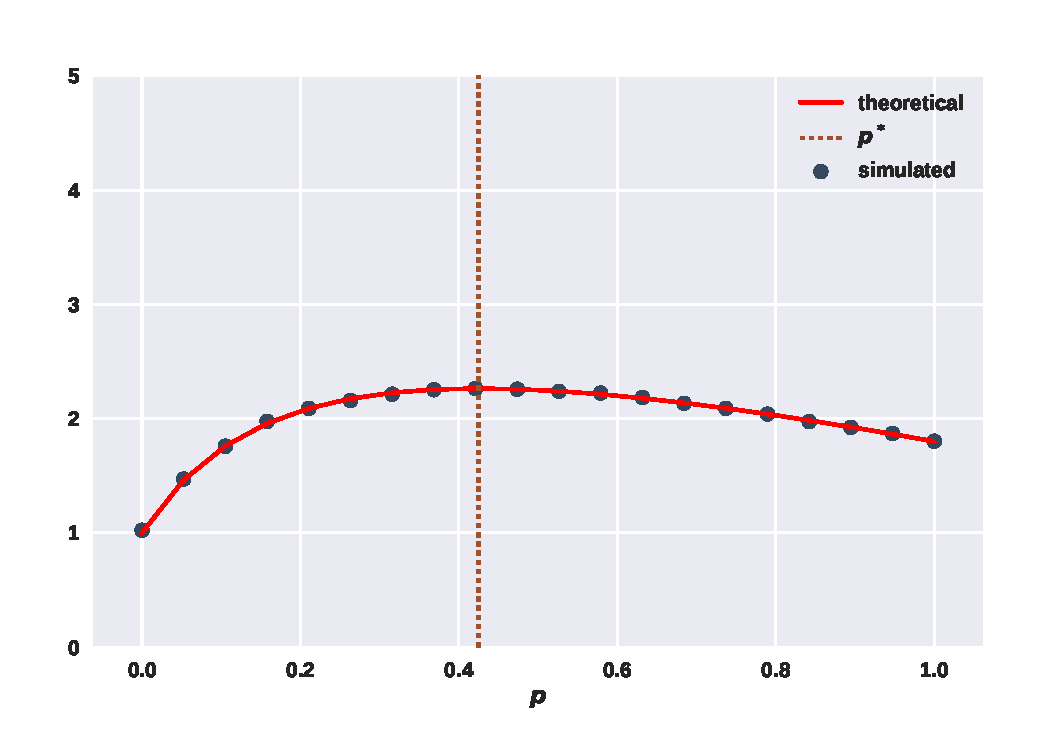
\includegraphics[width=.95\textwidth]{img/match_random}
    \end{subfigure}
    \begin{subfigure}{0.45\textwidth}
        \centering
        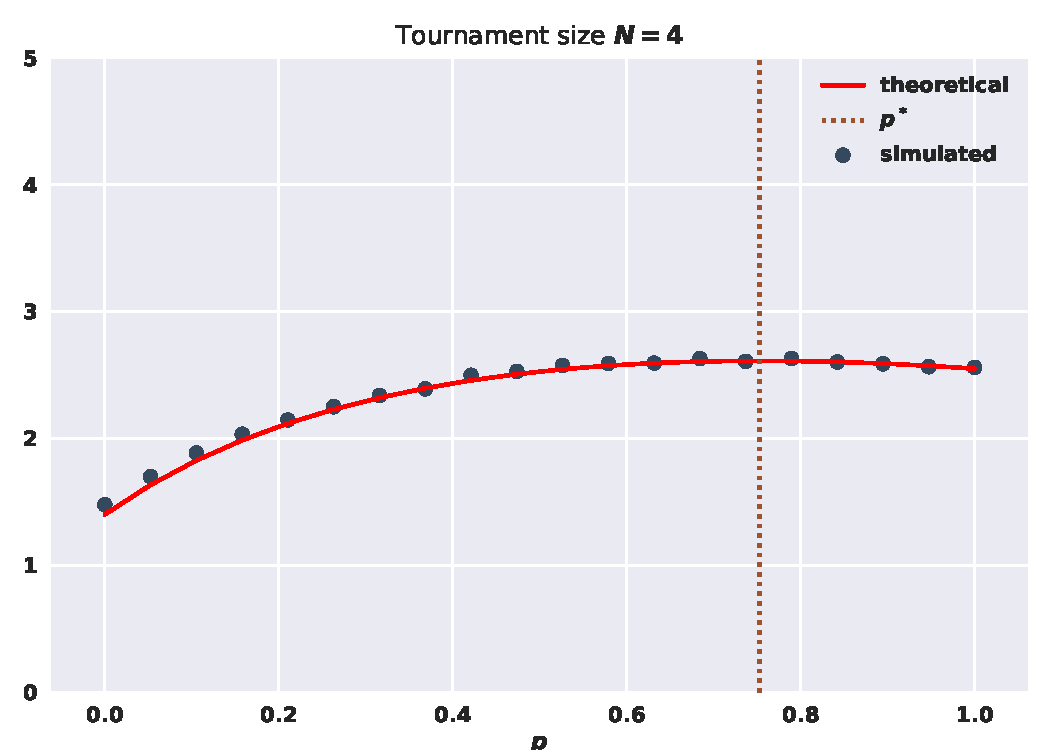
\includegraphics[width=.85\textwidth]{img/tournament_random}
    \end{subfigure}
    \caption{Numerical experiments for algorthim~\ref{algo:purely}.}
    \label{fig:purely_random_results}
\end{figure}

For the case of the purely random players two more theoretical results are discussed.
These are the cases where:

\begin{itemize}
    \item the oppponent has manage to make us indifferent
    \item the best behaviour is pure strategy.
\end{itemize}

The results are given equivilently by Lemmas~\ref{lemma:constant} and~\ref{lemma:linear}
and they are respective to the actions of the opponent.

\begin{lemma}\label{lemma:constant}
    A given memory one player, \((q_1, q_2, q_3, q_4)\), makes a \textbf{purely
    random} player, \((p, p, p, p)\), indifferent if and only if, 
    \(-q_1 + q_2 + 2q_3 - 2q_4 = 0 \) and 
    \((q_2 - q_4 - 1)(q_1 - 2q_2 - 5q_3 + 7q_4 + 1) -(q_2 - 5q_4 - 1)(q_1 - q_2 - q_3 + q_4) = 0 \).
\end{lemma}

\begin{lemma}\label{lemma:linear}
    Against a memory one player, \((q_1, q_2, q_3, q_4)\), a \textbf{purely random}
    player would always play a pure strategy if and only if
    \((q_{1}q_{4} - q_{2} q_{3} + q_{3} - q_{4}) (4 q_{1} - 3 q_{2} - 4 q_{3} + 3 
    q_{4} - 1) = 0\).
\end{lemma}

Reactive strategies are a set of memory one strategies where they only take into
account the opponents's previous moves. The optimisation problem of (\ref{eq:mo_optimisation})
now has an extra constraint and is re written as,

\begin{equation}\label{eq:random_optimisation}
\begin{aligned}
\max_p: & \ u_q(p)
\\
\text{such that}: & \ p_1 = p_3 \text{ and } p_2 = p_4\\
    & \ 0 \leq p_1, p_2 \leq 1.
\end{aligned}
\end{equation}

The following algorithm is used.

Note that resultant theory is a field of algebraic geometry and Sylvester's formulation
is a common resultant used for systems of 2 equations.
We suggested that several other resultant can be used here but Sylberster; has been used for simplisiti and 
speed reasons.

A numerical experiment suggests that the best response behvaiour is captured by our algorithm.

The numerical methods
results.

\section{Limitation of memory}

\section{Stability of defection}

% Bibliography
\bibliographystyle{plain}
\bibliography{bibliography.bib}

\end{document}
